\label{chap:kapitel3_3}
\section{Algorithmus von Reingold und Tilford}

Das Paper “Tidier Drawings of Trees” von Edward M. Reingold und John S. Tilford aus dem Jahre 1981,
welches im IEEE Transaction on Software Engineering erschienen ist, handelt von einem Algorithmus zum Zeichnen von Bäumen im Ebenen-Layout\cite[]{q2}.
Die Motivation der beiden Autoren für das Erstellen dieses Algorithmus beruht darauf, dass sie ein entscheidendes Problem an dem 
verbesserten Algorithmus von Wetherell und Shannon erkannt haben. Dieser Algorithmus ohne die Modifikation produziert Bäume, 
welche nicht maximal schmal sind, da das Zentrieren der Väter erzwungen wird. Die modifizierte Variante des 
Algorithmus produziert zwar maximal schmale Bäume, dafür können diese wesentlich unübersichtlicher sein, 
was der untere Baum auf Abbildung \ref{pic:baum_theorem_uglification} zeigt. 
Reingold und Tilford erkennen, dass das Problem an dem Algorithmus ist, dass die einzelnen Teilbäume von Knoten außerhalb des Teilbäume 
beeinflusst werden. Daraus folgern die beiden, dass es mit dem Algorithmus von Wetherell und Shannon dazu kommen kann, dass ein Baum und 
die Spiegelung desselben Baumes keine Spiegelbilder ergeben. Jedoch wäre es nach Reingold und Tilford wünschenswert, wenn symmetrische Bäume 
auch symmetrisch gezeichnet werden. Daraus wird eine weitere Anforderung an Algorithmen zum Zeichnen von Bäumen abgeleitet \cite[]{q2}.

\begin{quotation}
	\textit{Aesthetic 4:} A tree and its mirror image should produce
    drawings that are reflections of one another; moreover, a subtree
    should be drawn the same way regardless of where it
    occurs in the tree \cite[]{q4}.
\end{quotation}

Wenn der Algorithmus eine Spiegelung eines Baumes erhält und der durch den Algorithmus gezeichnete Baum ein exaktes Spiegelbild des 
eigentlichen Baumes ist, dann ist diese Anforderung erfüllt. Abbildung \ref{pic:WS_Spiegel} zeigt einen Baum und seine Spiegelung der mit 
unserer Implementierung des Algorithmus von Wetherell und Shannon gezeichnet wurde. Abbildung \ref{pic:TR_Spiegel} zeigt den selben Baum mit 
seiner Spiegelung, aber dieses mal mit unserer Java-Implementierung von Reingold und Tilfords Algorithmus. Zu erkennen an dieser Abbildung ist, 
dass der Algorithmus von Reingold und Tilford Aesthetic 4 erfüllt, der Algorithmus von Wetherell und Shannon jedoch nicht. Außerdem sollen 
Teilbäume immer gleich gezeichnet werden, unabhängig von ihrer Position im Baum.

Um diese Anforderung zu erfüllen, dürfen Knoten außerhalb eines Teilbaums die Knoten innerhalb eines Teilbaums nicht beeinflussen. 
Damit das erreicht wird, werden bei diesem Algorithmus nicht einzelne Knoten platziert (wie bei Wetherell und Shannon), 
sondern es werden zwei Teilbäume unabhängig voneinander platziert und dann so nah wie möglich aneinander geschoben \cite[]{q2}. 

\label{chap:kapitel3_3_Ablauf}
\subsection{Ablauf}

\begin{figure}[ht]
    \centering
    \begin{minipage}[]{0.3\linewidth}
        \centering
        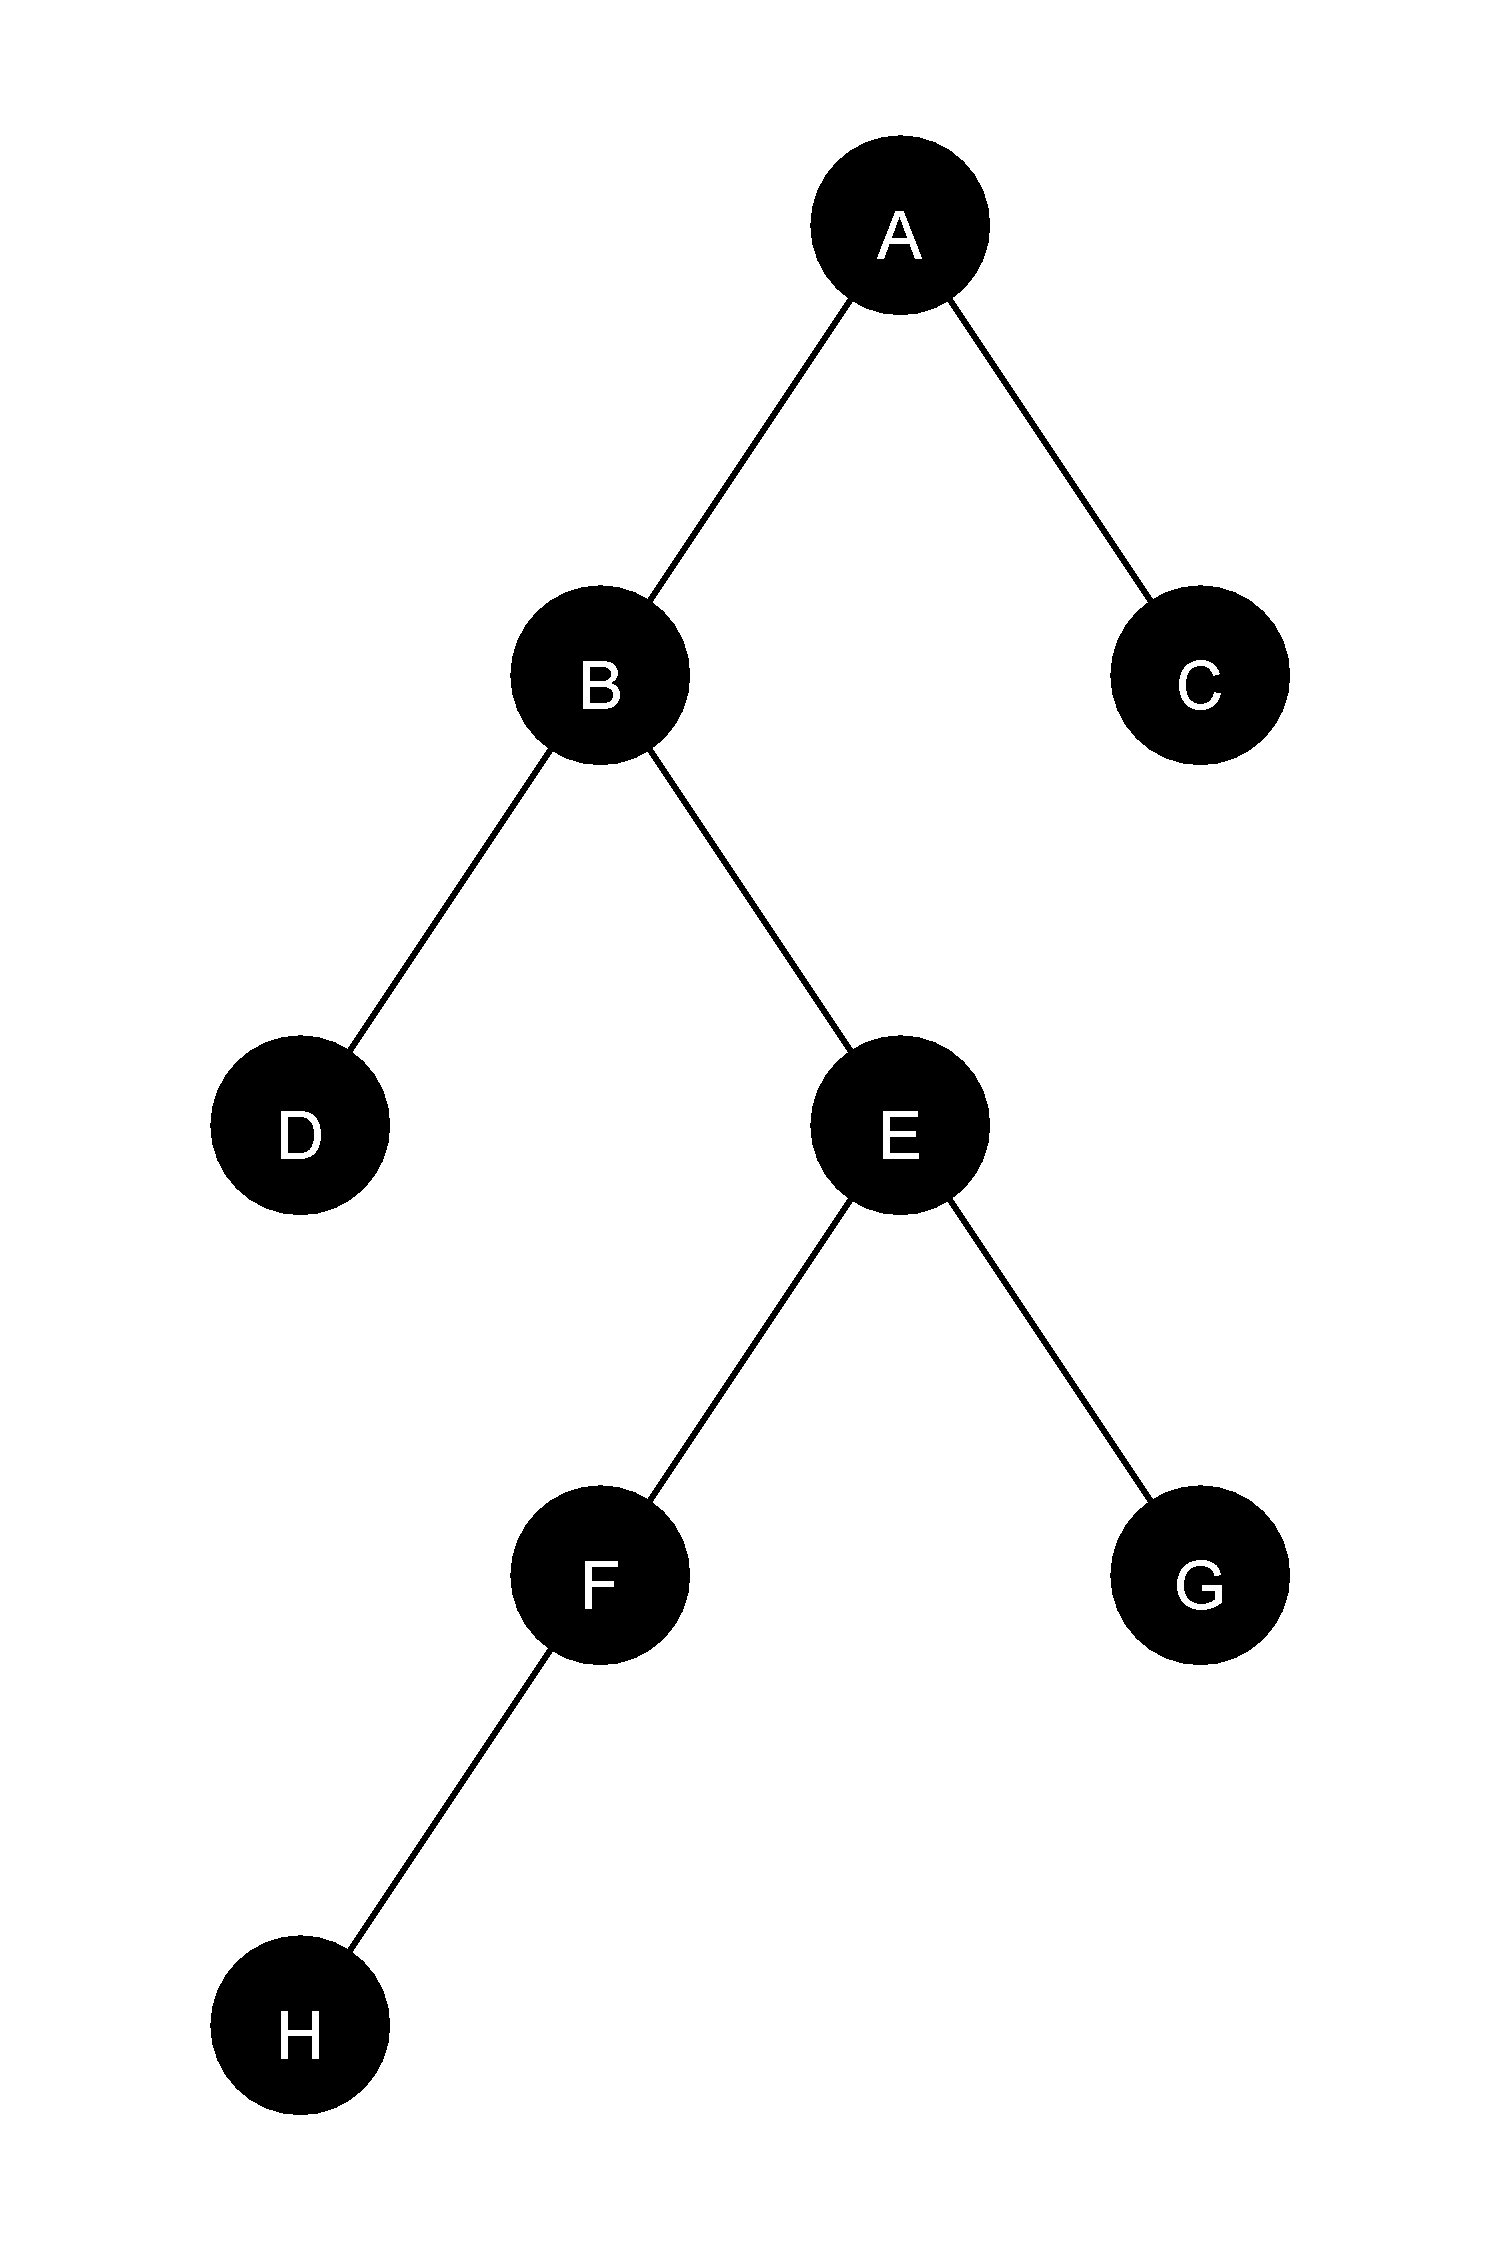
\includegraphics[scale=0.07]{abbildungen/tree_beispiel_LL_LR_RL_RR}
    \end{minipage}
    \hfill
    \begin{minipage}[]{0.65\linewidth}
        \centering
        \begin{tabular}{l | c | c | c | c | c | c | c | c}
            & A & B & C & D & E & F & G & H \\
            \hline\hline
            \textbf{LL} & H & D & C & D & H & H & G & H \\
            \textbf{LR} & G & D & C & D & F & H & G & H \\
            \textbf{RL} & C & H & C & D & G & H & G & H \\
            \textbf{RR} & C & G & C & D & G & H & G & H \\
            \end{tabular}
    \end{minipage} 
    \caption{Beispielhafte Bestimmung für \ac{LL}, \ac{LR}, \ac{RL}, \ac{RR}}
\end{figure}

Der Algorithmus zum Zeichnen von Bäumen von Reingold und Tilford lässt sich in zwei Phasen unterteilen.
Den ersten Teil stellt die Prozedur “Setup” dar. Diese Prozedur erhält vier Eingabeparameter, nämlich einen Knoten (welche am Anfang 
die Wurzel ist), die Höhe des Knotens im Gesamtbaum, sowie RMOST und LMOST. RMOST und LMOST sind jedoch nicht vom Datentyp Knoten, sondern 
von einem neuen Datentyp namens Extreme. Extreme sind Strukturen, die drei Attribute besitzen: 
\begin{itemize}
    \item Verweis auf einen Knoten
    \item Offset von der X-Koordinate zur Wurzel des Teilbaums
    \item Höhe des Knotens im Gesamtbaum
\end{itemize}

Zu Beginn der Prozedur wird geprüft, ob der übergebene Knoten NULL ist. Wenn dies nicht der Fall ist, 
dann wird die Y-Koordinate des Knotens auf seine Höhe gesetzt. Danach wird die Prozedur rekursiv aufgerufen, 
um eine Post-Order Traversierung auszuführen. Dieser Aufruf sieht wie folgt aus:

\begin{lstlisting}[caption = Rekursiver Aufruf von Setup]
    SETUP (L, LEVEL+1, LR, LL );
    SETUP (R, LEVEL+1, RR, RL );
\end{lstlisting}

Durch die Post-Order Traversierung wird die Setup Prozedur solange aufgerufen, bis der aktuelle Knoten das Blatt unten links ist. 
Da ein Blatt automatisch der am weitesten links und am weitesten rechts stehende Knoten ist, werden die Adressen von 
RMOST und LMOST auf diesen Knoten gesetzt. Außerdem wird die Höhe von RMOST und LMOST auf die Höhe des aktuellen Knotens gesetzt. 
Zudem werden die Offsets des Knotens und von RMOST sowie LMOST auf null gesetzt. 

Wenn der Knoten sowohl ein linkes als auch ein rechtes Kind hat, dann wird geprüft, ob das linke Kind ein rechtes Kind hat. 
Ist dies der Fall, dann wird der Offset des linken Kindes auf die Summe der linken Offsets addiert und vom aktuellen Abstand abgezogen. 
Zudem wird dann der Zeiger auf das linke Kind auf das rechte Kind des linken Kindes gesetzt. Andernfalls, wird dann der Offset des linken 
Kindes von der Summe der linken Offsets subtrahiert und der aktuelle Abstand um den Offset des linken Kindes erhöht. Auch wird danach der 
Zeiger auf das linke Kind auf das linke Kind des linken Kindes gesetzt. Genau dasselbe wird auch für das rechte Kind geprüft und ausgeführt. 
Falls danach der aktuelle Abstand kleiner als ein vorher festgelegter Mindestabstand ist, wird der Abstand zwischen den Kindern um den 
Mindestabstand minus dem aktuellen Abstand erhöht. Außerdem wird der aktuelle Abstand dann auf den Mindestabstand gesetzt. Dies wird solange 
ausgeführt, bis einer der beiden Zeiger (auf linkes/rechtes Kind) gleich NULL ist. Diese Schleife sorgt dafür, dass entlang der rechten 
Kontur des linken Teilbaums und entlang der linken Kontur des rechten Teilbaums die Distanz zwischen den beiden bestimmt wird. 
Gegebenenfalls werden dann die beiden Teilbäume auseinander geschoben, falls sie sich berühren \cite{q2}.

Nach dieser Schleife wird der Offset des aktuellen Knotens auf die Hälfte des Abstandes zwischen den Kindern plus eins gesetzt. 
Dieser Offset wird dann von der Summe der linken Offsets abgezogen und auf die Summe der rechten Offsets addiert. 

Danach werden RMOST und LMOST mit Hilfe von \ac{LL}, \ac{LR}, \ac{RL} und \ac{RR} neu festgelegt. Wenn die Höhe von \ac{RL} größer als die Höhe von \ac{LL} ist oder 
der aktuelle Knoten kein linkes Kind hat, dann setze LMOST auf \ac{RL} und erhöhe den Offset von LMOST um den Offset des Knotens. 
Ansonsten setze LMOST auf \ac{LL} und ziehe vom Offset von LMOST den Offset des Knotens ab. Diese Abfrage wird für RMOST und \ac{LR} sowie \ac{RR} 
wiederholt. Es wird geprüft, ob die Höhe von \ac{LR} größer ist als die Höhe von \ac{RR} oder der Knoten kein rechtes Kind hat. Wenn dies der Fall ist, 
dann wird RMOST auf \ac{LR} gesetzt und der Offset von RMOST um den Offset des Knotens verringert. Tritt dieser Fall nicht ein, dann wird RMOST 
auf \ac{RR} gesetzt und der Offset von RMOST mit dem Offset des Knotens addiert. 

RMOST und LMOST korrekt festzulegen ist für den nächsten Schritt wichtig und notwendig. Diese beiden Knoten in einem Subtree 
sind die einzigen, bei denen die Möglichkeit besteht, dass Threading angewandt wird. Dieser Schritt ist nur dann nötig, wenn 
die beiden betrachteten Teilbäume eines Knotens unterschiedlich hoch sind und keiner von beiden leer ist. Reingold und Tilford 
geben dafür ein Beispiel an. Wenn der linke Subtree höher als der rechte Subtree ist, dann muss ein Thread von \ac{RR} zu dem am weitesten 
rechts stehenden Knoten des linken Teilbaums auf der nächsten Höhe gelegt werden. Dieser Thread würde in dem Zeiger auf das linke Kind 
von \ac{RR} gespeichert werden. Benötigt werden diese Threads als eine Art “Pseudo-Kante” um sicherzustellen, dass diese Teilbäume sich 
nicht berühren und auseinander geschoben werden.

Die zweite Phase des Algorithmus stellt die Prozedur “petrify” dar. Ziel dieser Prozedur ist es die relativen Offsets, 
welche in der vorherigen Phase gesetzt worden, in absolute Koordinaten umzuwandeln. Zudem sorgt die Prozedur dafür, dass die Threads 
gelöscht werden, da diese nicht mehr benötigt werden. Um dies zu erreichen wird eine Pre-Order-Traversierung 
über dem Baum durchgeführt. Dafür bekommt “petrify” zwei Eingabeparameter, nämlich einen Knoten (zu Beginn wieder die Wurzel) und eine 
initiale X-Position (ist beliebig). Dann prüft die Prozedur, ob der Knoten ungleich NULL ist. Wenn dies der Fall ist, dann wird geschaut, 
ob der Knoten einen Thread hat. Da Threads Blätter sein müssen, werden die Verweise des Knotens auf sein linkes und rechtes Kind gelöscht, 
um keinen Thread fälschlicherweise als Kante darzustellen. Dann setzt die Prozedur die finale X-Koordinate des Knotens auf den 
übergebenen Parameter. Zum Schluss wird “petrify” wie folgt rekursiv aufgerufen:

\begin{lstlisting}[caption=Rekursiver Aufruf von Petrify (Pre-Order)]
    PETRIFY(T.LLINK, XPOS - T.OFFSET);
    PETRIFY(T.RLINK, XPOS + T.OFFSET);
\end{lstlisting}

Bei linken Kindern wird der Offset des Vaters von der X-Koordinate abgezogen. Bei rechten Kindern wird dann die X-Koordinate mit dem 
Offset des Vaters addiert. Ziel dessen ist, dass linke Kind links vom Vater und rechte Kinder rechts vom Vater stehen.


\subsection{Implementierung in Java}

\begin{figure}[H]
    \centering
    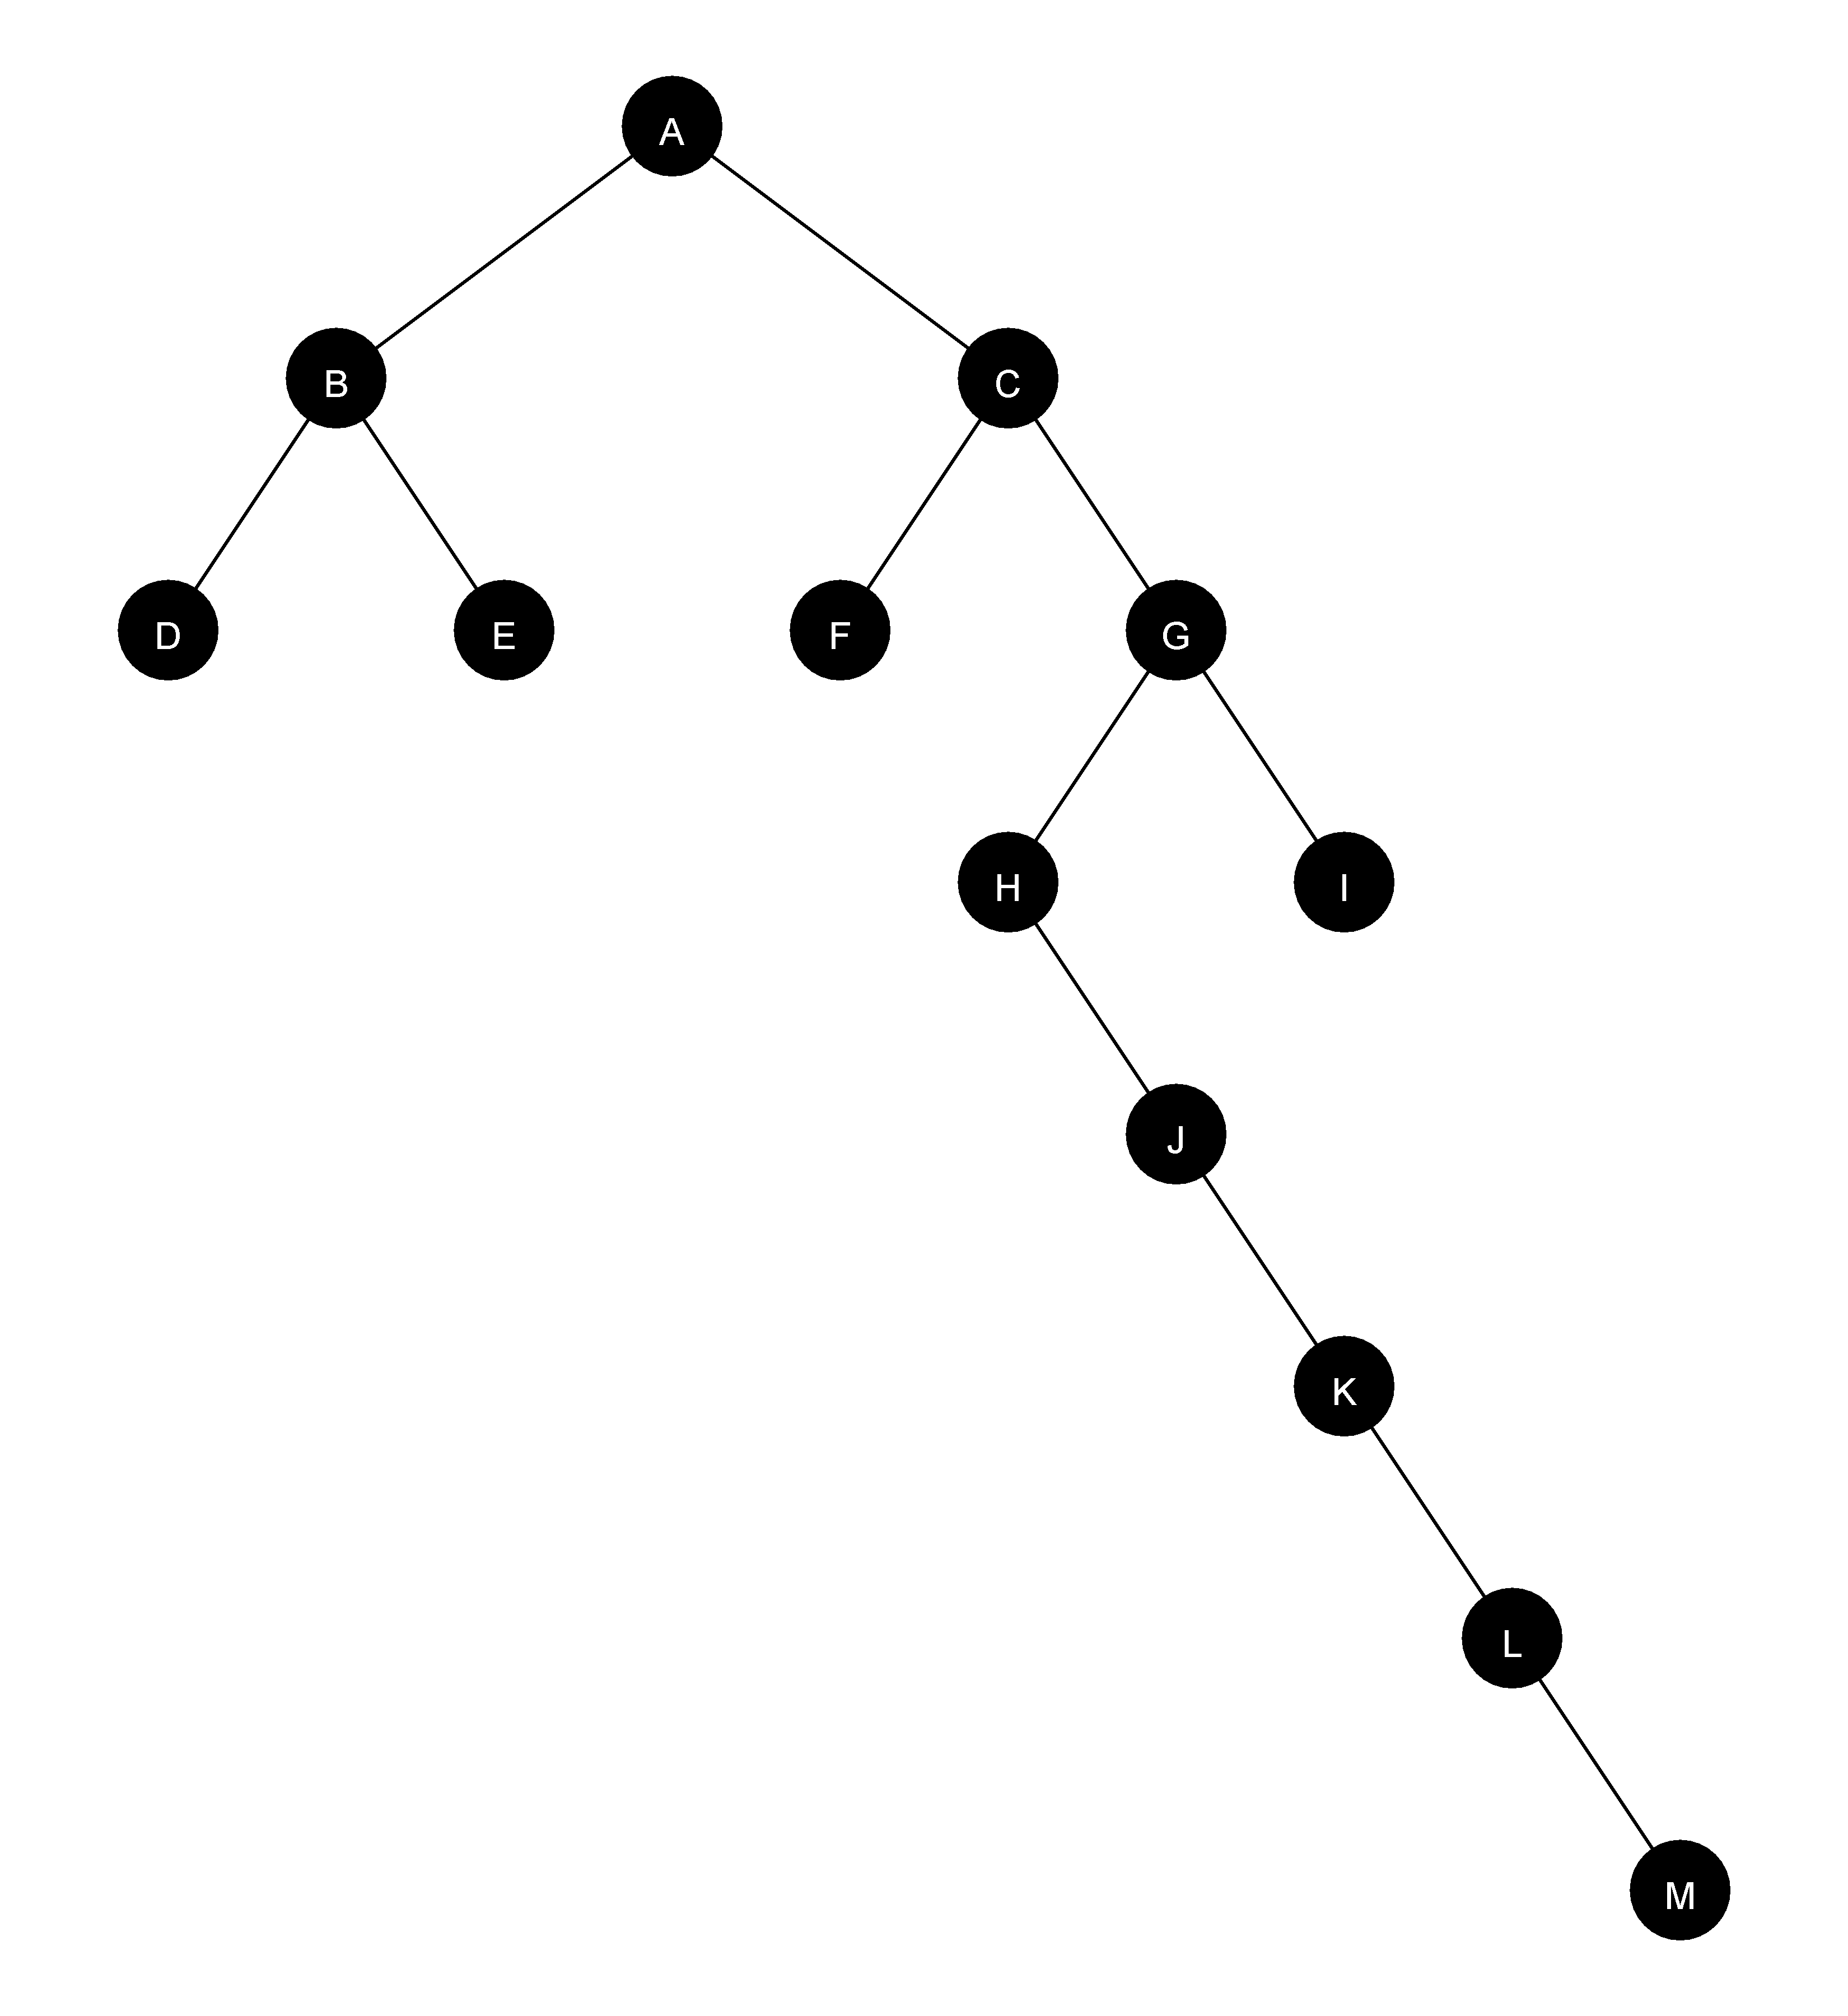
\includegraphics[scale = 0.05]{abbildungen/baum_algo_3_n1}
    \caption{Gezeichneter komplexer Baum durch den Tilford Algorithmus}
    \label{pic:baum_algo_3_n1} 
\end{figure}

\begin{figure}[H]
    \centering
    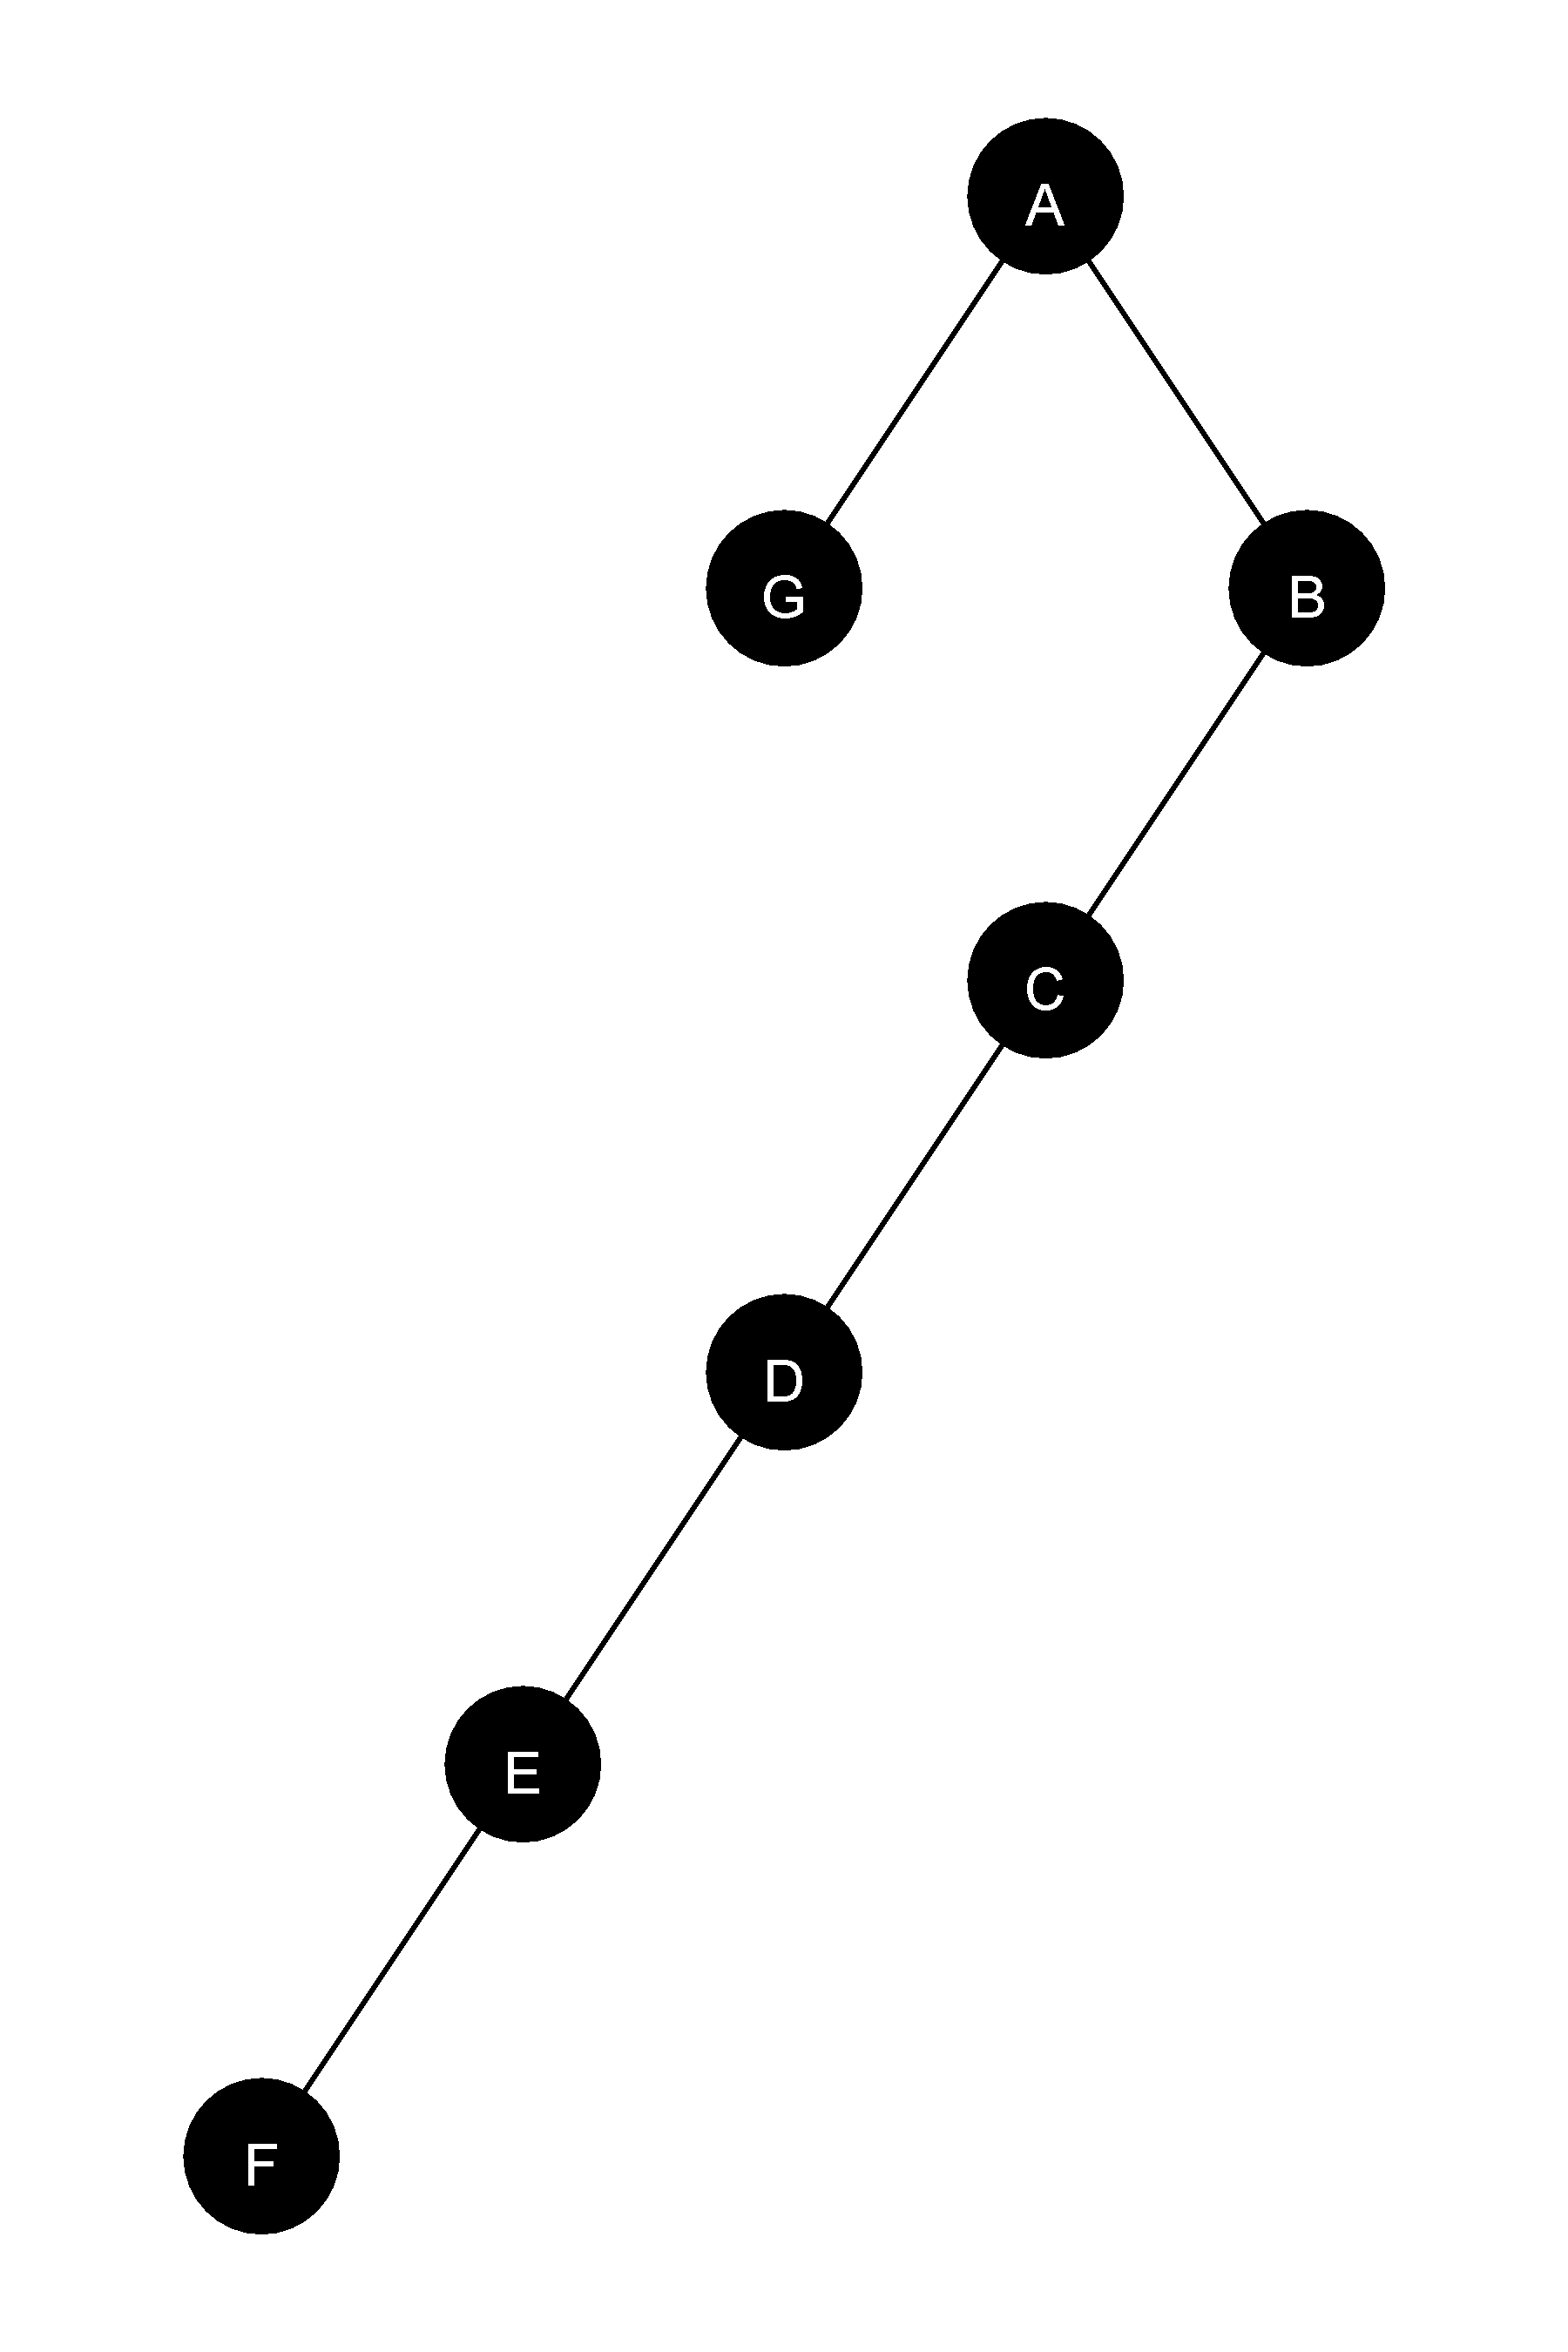
\includegraphics[scale = 0.07]{abbildungen/baum_algo_3_n2}
    \caption{Gezeichneter einfacher Baum durch den Tilford Algorithmus}
    \label{pic:baum_algo_3_n2} 
\end{figure}

Um diesen Algorithmus implementieren zu können, muss die zuvor erstellte BinaryKnoten-Klasse um ein 
Attribut erweitert werden: vom Typ Boolean mit dem Namen \glqq thread\grqq. Zudem wurde eine weitere Klasse 
namens \glqq Extreme\grqq definiert, die wie zuvor beschrieben, implementiert wurde. Die Extreme-Klasse sieht wie folgt aus:

\begin{lstlisting}[caption=Implementierung der Extreme-Klasse, label=code:algo3_extreme]
private static class Extreme {
    BinaryKnoten knoten;
    int offset;
    int level;
    
    void set(BinaryKnoten k, int offset) {
        this.knoten = k;
        this.level = k.getHoehe();
        this.offset = offset;
    }
}
\end{lstlisting}

Ferner wurden die zuvor beschriebenen Prozeduren \glqq setup\grqq und \glqq petrify\grqq implementiert. Die implementierte Prozedur
\glqq setup\grqq unterscheidet sich zum zuvor beschriebenen Ablauf. Sie wird nun nicht mehr rekursiv aufgerufen und besitzt 
nur einen Eingabeparameter, den Wurzelknoten. Hiernach wird mithilfe der \glqq traversPostOrder\grqq-Methode aus der 
BinaryKnoten-Klasse über den Baum traversiert.

\begin{lstlisting}[caption=Ausschnitt aus der setup-Prozedur, label=code:algo3_setup]
public static void setup(BinaryKnoten wurzel) {
    // Initialisierungen von Variablen
    // <...>
    // Ueber den Baum in der Post-Order traversieren
    wurzel.traversPostOrder(k -> {
        BinaryKnoten knoten = (BinaryKnoten) k;

        // Bestimmen der Y-Koordinate
        knoten.setY(2 * knoten.getHoehe() + 1);

        // Vorlaeufige relative X-Koordinate bestimmem
        // <...>
    }
}
\end{lstlisting}

Abweichend zum Ablauf entspricht die Y-Koordinate nicht der Höhe des Knotens. Stattdessen wird diese wie im 
Ablauf aus dem Kapitel \ref{chap:kapitel3_1_Ablauf} berechnet. Dies bietet den Vorteil, 
dass die Methodik zum Zeichnen der Bäume nicht verändert werden muss. Die weitere Implementierung folgt 
der Beschreibung aus dem Ablauf.

Die Implementierung der Prozedur \glqq petrify\grqq entspricht der Beschreibung aus dem Ablauf.

Hiernach wurde die Prozedur \glqq algorithmus3\grqq definiert. Diese ruft zu Beginn die beiden Prozeduren, 
\glqq setup\grqq und \glqq petrify\grqq auf. Danach müssen die X-Koordinaten noch angepasst werden, da diese 
negativ sein können. Hierfür wird der kleinste X-Wert ermittelt, dessen absoluter Wert 
addiert mit eins in der Variable \glqq offset\grqq gespeichert wird. Nun werden alle X-Koordinaten des 
Baums mit dem Wert aus \glqq offset\grqq addiert. 

Zwei beispielhafte Ergebnisse können in den Abbildungen \ref{pic:baum_algo_3_n1} 
und \ref{pic:baum_algo_3_n2} betrachtet werden. 


\subsection{Vor- und Nachteile}

Ein Algorithmus, welcher Aesthetic 4 erfüllt, kann Bäume produzieren, welche nicht maximal schmal sind. 
Für Reingold und Tilford ist das Erfüllen dieser Anforderung jedoch wichtiger als das Einhalten des physikalischen Limits, 
da Aesthetic 4 dafür sorgt, dass diese Bäume für Menschen übersichtlicher und leichter zu verstehen sind \cite[]{q2}. Dafür ist der Algorithmus 
jedoch, gemessen an den Zeilen im Programmcode, der längste. Selbst bei komplexeren Bäumen, wie in Abbildung \ref{pic:baum_algo_3_n2},
wird ein übersichtlicher und ästhetisch ansprechender Baum gezeichnet. 

Ähnlich wie der verbesserte Algorithmus von Wetherell und Shannon ist der Algorithmus von Reingold und Tilford so wie er ist nur in Lage
Binärbäume zu zeichnen. Jedoch beschreiben die beiden Autoren wie der Algorithmus modifiziert werden kann um beliebige Bäume zu zeichnen.

